\documentclass[12pt,a4paper]{article}
\usepackage{amsmath,amscd,amsbsy,amssymb,latexsym,url,bm,amsthm}
\usepackage{epsfig,graphicx,subfigure}
\usepackage{enumitem,balance}
\usepackage{wrapfig}
\usepackage{mathrsfs,euscript}
\usepackage[usenames]{xcolor}
\usepackage{hyperref}
\usepackage[vlined,ruled,linesnumbered]{algorithm2e}
\usepackage{array}
\hypersetup{colorlinks=true,linkcolor=black}
\usepackage{attachfile}
\usepackage{listings}

\newtheorem{theorem}{Theorem}
\newtheorem{lemma}[theorem]{Lemma}
\newtheorem{proposition}[theorem]{Proposition}
\newtheorem{corollary}[theorem]{Corollary}
\newtheorem{exercise}{Exercise}
\newtheorem*{solution}{Solution}
\newtheorem{definition}{Definition}
\theoremstyle{definition}

\renewcommand{\thefootnote}{\fnsymbol{footnote}}

\newcommand{\postscript}[2]
 {\setlength{\epsfxsize}{#2\hsize}
  \centerline{\epsfbox{#1}}}

\renewcommand{\baselinestretch}{1.0}

\setlength{\oddsidemargin}{-0.365in}
\setlength{\evensidemargin}{-0.365in}
\setlength{\topmargin}{-0.3in}
\setlength{\headheight}{0in}
\setlength{\headsep}{0in}
\setlength{\textheight}{10.1in}
\setlength{\textwidth}{7in}
\makeatletter \renewenvironment{proof}[1][Proof] {\par\pushQED{\qed}\normalfont\topsep6\p@\@plus6\p@\relax\trivlist\item[\hskip\labelsep\bfseries#1\@addpunct{.}]\ignorespaces}{\popQED\endtrivlist\@endpefalse} \makeatother
\makeatletter
\renewenvironment{solution}[1][Solution] {\par\pushQED{\qed}\normalfont\topsep6\p@\@plus6\p@\relax\trivlist\item[\hskip\labelsep\bfseries#1\@addpunct{.}]\ignorespaces}{\popQED\endtrivlist\@endpefalse} \makeatother

\begin{document}
\noindent

%========================================================================
\noindent\framebox[\linewidth]{\shortstack[c]{
\Large{\textbf{Lab06-Linear Programming}}\vspace{1mm}\\
CS214-Algorithm and Complexity, Xiaofeng Gao, Spring 2021.}}
\begin{center}
\footnotesize{\color{red}$*$ If there is any problem, please contact TA Haolin Zhou.}

% Please write down your name, student id and email.
\footnotesize{\color{blue}$*$ Name:\underline{Xin Xu}  \quad Student ID:\underline{519021910726} \quad Email: \underline{xuxin20010203@sjtu.edu.cn}}
\end{center}

\begin{enumerate}
    \item
    \textit{Hirschberg Algorithm.} Recall the \textbf{String Similarity} problem in class, in which we calculate the edit distance between two strings in a sequence alignment manner.
    \begin{enumerate}
    	\item
    	Implement the algorithm combining \textbf{dynamic programming} and \textbf{divide-and-conquer} strategy in C/C++. Analyze the time complexity of your algorithm. {\color{blue}(The template \emph{Code-SequenceAlignment.cpp} is attached on the course webpage)}.
    	
    	\item
    	Given $\alpha(x, y) = |ascii(x) - acsii(y)|$, where $ascii(c)$ is the ASCII code of character $c$, and $\delta=13$. Find the edit distance between the following two strings.
    	\begin{align*}
    		X[1..60]=&\ CMQHZZRIQOQJOCFPRWOUXXCEMYSWUJ\\
    		&\ TAQBKAJIETSJPWUPMZLNLOMOZNLTLQ	
    	\end{align*}
    	\begin{align*}
    		Y[1..50]=&\ SUYLVMUSDROFBXUDCOHAATBKN\\
    		&\ AAENXEVWNLMYUQRPEOCJOCIMZ
    	\end{align*}
    \end{enumerate}

    \begin{solution}
      \begin{enumerate}
        \item Let $T(m,n)$ be the max running time of algorithm on strings of length $m$ and $n$. We know from the algorithm that $T(m,n)\leqslant cmn+T(q,n/2)+T(m-q,n/2)$. We assume that $T(m,n)=O(mn)$ for any integers $m,n\leqslant 2$ with the conditions $T(m,2)\leqslant cm;T(2,n)\leqslant cn$. 
        \\ $T(m,n)\leqslant cmn+T(q,n/2)+T(m-q,n/2)$
        \\ $\leqslant 2cqn/2+2c(m-q)n/2+cmn$
        \\ $=cqn+cmn-cqn+cmn$
        \\ $=2cmn$
        \\So, the time complexity is $O(mn)$.
        \item The answer is 385. More details are in .cpp file.
      \end{enumerate}
    \end{solution}
    
    \item 
    \textit{Travelling Salesman Problem.} Given a list of cities and the distances between each pair of cities ($ G=(V,E,W) $), we want to find the shortest possible route that visits each city exactly once and returns to the origin city. Similar to \textbf{Maximum Independent Set} and \textbf{Dominating Set}, please turn the traveling salesman problem into an ILP form.  
    
    \textbf{Remark:} $ W $ is the set of weights corresponds to the edges that connecting adjacent cities.  
    \begin{solution}
      We construct two matrices $A$ and $W$, and
      $$ a_{ij}=\left\{
      \begin{aligned}
      1 \text{ if the route includes a path from }v_i\text{ to }v_j \\
      0 ,\text{ else}
      \end{aligned}
      \right.
      $$
      $$ w_{ij}=\left\{
      \begin{aligned}
      w_{ij} \text{ if the route includes a path from }v_i\text{ to }v_j\text{ with the weight of }w_{ij} \\
      0 ,\text{ else}
      \end{aligned}
      \right.
      $$
      The ILP form is:
      \\minimize the sum of elements on the diagonal of $A\times W$.
      \\The sum of each row and the sum of each column are both 1.
    \end{solution}
    \item
    \textit{Investment Strategy.} A company intends to invest $0.3$ million yuan in $2021$, with a proper combination of the following $3$ projects:
    \begin{itemize}
    \item \textbf{Project 1:} Invest at the beginning of a year, and can receive a $20\%$ profit of the investment in this project at the end of this year. Both the capital and profit can be invested at the beginning of next year;
    \item \textbf{Project 2:} Invest at the beginning of $2021$, and can receive a $50\%$ profit of the investment in this project at the end of $2022$. The investment in this project cannot exceed $0.15$ million dollars;
    \item \textbf{Project 3:} Invest at the beginning of $2022$, and can receive a $40\%$ profit of the investment in this project at the end of $2022$. The investment in this project cannot exceed $0.1$ million dollars.
    \end{itemize}
    Assume that the company will invest \emph{all} its money at the beginning of a year. Please design a scheme of investment in $2021$ and $2022$ which maximizes the overall sum of capital and profit at the end of $2022$.
    \begin{enumerate}
    \item
    Formulate a linear programming with necessary explanations.

    \item
    Transform your LP into its standard form and slack form.

    \item
    Transform your LP into its dual form.

    \item
    Use the simplex method to solve your LP.
    \end{enumerate}
    
    \begin{solution}
      \begin{enumerate}
        \item Let $x_1$ be the investment to project 2, $x_2$ be the investment to project 1 in the first year, $x_3$ be the investment to project 3 in the second year, and $x_4$ be the investment to project 1 in the second year.
        \\ The linear programming is:
        \\ max $1.5x_1+1.4x_3+1.2x_4$
        \\$x_1+x_2=0.3, x_3+x_4=1.2x_2, x_1\leqslant 0.15, x_3\leqslant 0.1, x_1\geqslant 0, x_2\geqslant 0, x_3\geqslant 0, x_4\geqslant 0$.
        \item standard form:
        \\ max $1.5x_1+1.4x_3+1.2x_4$
        \\ $1.2x_1+x_3+x_4\leqslant 0.36$
        \\ $-1.2x_1-x_3-x_4\leqslant -0.36$
        \\ $x_1\leqslant 0.15$
        \\ $x_3\leqslant 0.1$
        \\ $x_1\geqslant 0, x_3\geqslant 0, x_4\geqslant 0$
        \\ slack form:
        \\ max $1.5x_1+1.4x_3+1.2x_4$
        \\ $1.2x_1+x_3+x_4 = 0.36$
        \\ $x_1 + x_5 = 0.15$
        \\ $x_3 + x_6 = 0.1$
        \\ $x_1\geqslant 0, x_3\geqslant 0, x_4\geqslant 0, x_5\geqslant 0, x_6\geqslant 0$
        \item dual form:
        \\ min $0.36y_1+0.15y_2+0.1y_3$
        \\ $1.2y_1+y_2\geqslant 1.5$
        \\ $y_1+y_3\geqslant 1.4$
        \\ $y_1\geqslant 1.2$
        \\ $y_1,y_2,y_3\geqslant 0$
        \item simplex method:
        \\ slack form:
        \\ max $1.5x_1+1.4x_3+1.2x_4$
        \\ $1.2x_1+x_3+x_4 = 0.36$
        \\ $x_1 + x_5 = 0.15$
        \\ $x_3 + x_6 = 0.1$
        \\ $x_1\geqslant 0, x_3\geqslant 0, x_4\geqslant 0, x_5\geqslant 0, x_6\geqslant 0$ 
        \\ The basic solution is $x=(0,0,0.36,0.15,0.1)$
        \\ Update $x_1$ to most: $x=(0.15,0,0.18,0,0.1)$
        \\ Update the function: max $0.225-1.5x_5+1.4x_3+1.2x_4$
        \\ Update $x_3$ to most: $x=(0.15,0.1,0.08,0,0)$
        \\ Update the function: max $0.365-1.5x_5-1.4x_6+1.2x_4$
        \\ The answer of this solution is $0.365+1.2*0.08=0.461$. Since one of the solutions to dual form is: $y=(1.2,0.06,0.2)$, min$=0.36*1.2+0.15*0.06+0.1*0.2=0.461$, 
        the solution is $x=(0.15,0.1,0.08,0,0)$, and the maximum of capital and profit is $0.461$.
      \end{enumerate}
    \end{solution}
    \item
    \textit{Factory Production.} An engineering factory makes seven products (PROD 1 to PROD 7) on the following machines: four grinders, two vertical drills, three horizontal drills, one borer and one planer. Each product yields a certain contribution to profit (in \pounds/unit). These quantities (in \pounds/unit) together with the unit production times (hours) required on each process are given below. A dash indicates that a product does not require a process.

    \begin{table}[htbp]
      \scriptsize
      \centering
      \renewcommand\arraystretch{1.1}
      \begin{tabular}{m{0.18\textwidth} m{0.07\textwidth}<{\centering} m{0.07\textwidth}<{\centering} m{0.07\textwidth}<{\centering} m{0.07\textwidth}<{\centering} m{0.07\textwidth}<{\centering} m{0.07\textwidth}<{\centering} m{0.07\textwidth}<{\centering}}
      \hline
       & \textbf{PROD 1} & \textbf{PROD 2} & \textbf{PROD 3} & \textbf{PROD 4} & \textbf{PROD 5} & \textbf{PROD 6} &  \textbf{PROD 7} \\\hline
      Contribution to profit & 10 & 6 & 8 & 4 & 11 & 9 & 3 \\
      Grinding & 0.5 & 0.7 & - & - & 0.3 & 0.2 & 0.5 \\
      Vertical drilling & 0.1 & 0.2 & - & 0.3 & - & 0.6 & - \\
      Horizontal drilling & 0.2 & - & 0.8 & - & - & - & 0.6 \\
      Boring & 0.05 & 0.03 & - & 0.07 & 0.1 & - & 0.08 \\
      Planing & - & - & 0.01 & - & 0.05 & - & 0.05 \\
      \hline
      \end{tabular}
    \end{table}

    There are marketing limitations on each product in each month, given in the following table:

    \begin{table}[htbp]
      \scriptsize
      \centering
      \renewcommand\arraystretch{1.1}
      \begin{tabular}{m{0.1\textwidth} m{0.07\textwidth}<{\centering} m{0.07\textwidth}<{\centering} m{0.07\textwidth}<{\centering} m{0.07\textwidth}<{\centering} m{0.07\textwidth}<{\centering} m{0.07\textwidth}<{\centering} m{0.07\textwidth}<{\centering}}
      \hline
       & \textbf{PROD 1} & \textbf{PROD 2} & \textbf{PROD 3} & \textbf{PROD 4} & \textbf{PROD 5} & \textbf{PROD 6} &  \textbf{PROD 7} \\\hline
      January & 500 & 1000 & 300 & 300 & 800 & 200 & 100 \\
      February & 600 & 500 & 200 & 0 & 400 & 300 & 150 \\
      March & 300 & 600 & 0 & 0 & 500 & 400 & 100 \\
      April & 200 & 300 & 400 & 500 & 200 & 0 & 100 \\
      May & 0 & 100 & 500 & 100 & 1000 & 300 & 0 \\
      June & 500 & 500 & 100 & 300 & 1100 & 500 & 60 \\
      \hline
      \end{tabular}
    \end{table}

    It is possible to store up to 100 of each product at a time at a cost of \pounds0.5 per unit per month (charged at the end of each month according to the amount held at that time). There are no stocks at present, but it is desired to have a stock of exactly 50 of each type of product at the end of June. The factory works six days a week with two shifts of 8h each day. It may be assumed that each month consists of only 24 working days. Each machine must be down for maintenance in one month of the six. No sequencing problems need to be considered.

    When and what should the factory make in order to maximize the total net profit?

    \begin{enumerate}
    \item
    Use \emph{CPLEX Optimization Studio} to solve this problem. Describe your model in \emph{Optimization Programming Language} (OPL). Remember to use a separate data file (.dat) rather than embedding the data into the model file (.mod).

    \item
    Solve your model and give the following results.
    \begin{enumerate}
    \item
    For each machine:
    \begin{enumerate}
    \item
    the month for maintenance.
    \end{enumerate}
    \item
    For each product:
    \begin{enumerate}
    \item
    The amount to make in each month.
    \item
    The amount to sell in each month.
    \item
    The amount to hold at the end of each month.
    \end{enumerate}
    \item
    The total selling profit.
    \item
    The total holding cost.
    \item
    The total net profit (selling profit minus holding cost).
    \end{enumerate}
    \end{enumerate}
    \textbf{Remark:} You can choose to use the attached .dat file or write it yourself. 

    \begin{solution}
      \begin{enumerate}
        \item .dat file and .mod file are in the folder.
        \item The answer of first two question is:
        \begin{figure}[htbp]
          \centering
          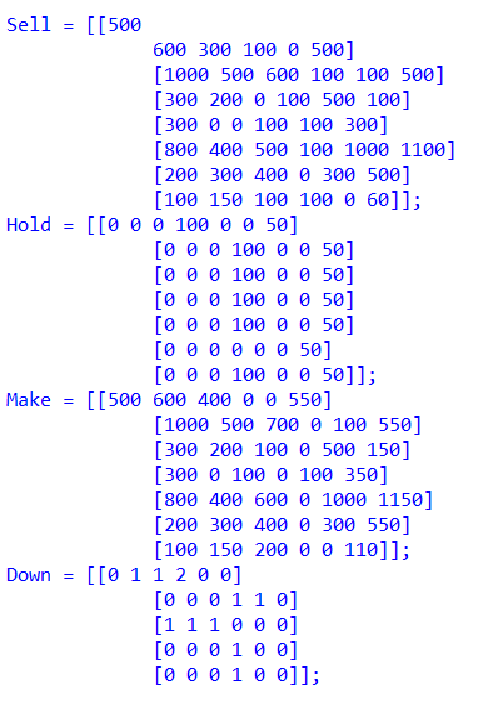
\includegraphics[width=0.4\textwidth]{machine and product.pdf}
          \caption{machine and product}\label{machine and product}
        \end{figure}
        
        \begin{figure}[htbp]
          \centering
          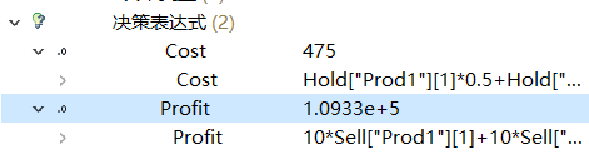
\includegraphics[width=0.4\textwidth]{cost and profit.pdf}
          \caption{cost and profit}\label{cost and profit}
        \end{figure}
      \end{enumerate}
    \end{solution}

\end{enumerate}
\newpage
\vspace{20pt}

{\noindent\large\textbf{Appendix}}
\begin{enumerate}
	\item [\textbf{A.}]
	\textbf{FactoryPlanning.dat}
	\attachfile{FactoryPlanning.dat}
	\lstset{
		language=C,
		tabsize=2,
		basicstyle=\footnotesize\ttfamily,
		columns=fullflexible,
		keywordstyle=\color{blue},
		numbers=left,
		numberstyle=\scriptsize\ttfamily,
		frame=single
	}
	\begin{lstlisting}
		NbMonths = 6;
		
		Prod = {Prod1, Prod2, Prod3, Prod4, Prod5, Prod6, Prod7};
		Process = {Grind, VDrill, HDrill, Bore, Plane};
		
		// profitProd[j] is profit per unit for product j
		ProfitProd = [10 6 8 4 11 9 3];
		
		// processProd[i][j] gives hours of process i required by product j
		ProcessProd = [[0.5  0.7  0.0  0.0  0.3  0.2 0.5 ]
		[0.1  0.2  0.0  0.3  0.0  0.6 0.0 ]
		[0.2  0.0  0.8  0.0  0.0  0.0 0.6 ]
		[0.05 0.03 0.0  0.07 0.1  0.0 0.08]
		[0.0  0.0  0.01 0.0  0.05 0.0 0.05]];
		
		// marketProd[i][j] gives marketing limitation on product j for month i
		MarketProd = [[500 1000 300  300 800  200 100]
		[600 500  200  0   400  300 150]
		[300 600  0    0   500  400 100]
		[200 300  400  500 200  0   100]
		[0   100  500  100 1000 300 0  ]
		[500 500  100  300 1100 500 60 ]];
		
		CostHold  = 0.5;
		StartHold = 0;
		EndHold   = 50;
		MaxHold   = 100;
		
		// process capacity
		HoursMonth = 384; // 2 eight hour shifts per day, 24 working days per month;
		
		// number of each type of machine
		NumProcess = [4 2 3 1 1];
		
		// how many machines must be down over 6 month period
		NumDown = [4 2 3 1 1];
	\end{lstlisting}
\end{enumerate}

\textbf{Remark:} You need to include your .cpp, .mod, .dat, .pdf and .tex files in your uploaded .zip file.



%========================================================================
\end{document}
